\documentclass{sig-alternate}

\newdef{defn}{Definition}
\newdef{conjecture}{Conjecture}

\newtheorem{theorem}{Theorem}
\newdef{case}{Case}
\newdef{remark}{Remark}

\usepackage{fourier}

\newcommand\npos[0]{\textbf{N}}
\newcommand\ppos[0]{\textbf{P}}

\usepackage{tikz}

\begin{document}

\title{Combinatorial Game Representation and Analysis of Snort}
\author{
	Gio Carlo C. Borje \\
	\affaddr{gborje@uci.edu} \\
	\affaddr{University of California, Irvine}
}
\maketitle

\begin{abstract}
The game of a Snort is a partisan, combinatorial game where solving which
player has a winning strategy is a \textbf{PSPACE}-complete problem. We
analyze the game of Snort by describing a state space prove that the game is
unfair. However, rather than solving the game for general graphs, we
demonstrate generalized winning strategies for a few common families of graphs
such as star graphs, path graphs and cycle graphs.
\end{abstract}

\section{Introduction}

The game of Snort, invented by Simon Norton, is a two-player game with a planar
map as a game board. The two players will be referred to as Red and Blue. The
red and blue players have distinct game pieces denoted by their corresponding
player's color. Players alternate turns placing pieces on the planar map with
two restrictions:
\begin{enumerate}
	\item Distinct game pieces cannot share a map position and
	\item Distinct game pieces cannot be in adjacent map positions.
\end{enumerate}
The game follows \emph{normal play} where the last player to move wins.

\subsection{Game Classification}

The game can be classified as follows:
\begin{description}
	\item [Determinate] No elements of chance are presented.
	\item [Zero-sum] No draws are possible.
	\item [Asymmetric] Each player can have different strategies.
	\item [Perfect information] No information of the game state is hidden from
		either player.
	\item [Sequential] Players alternate turns.
	\item [Normal-play] The last player to move wins the game.
	\item [Unfair] The game is unfair because a winning strategy exists for a
		player on any given game state.
\end{description}

Solving the winner of a given game state is a \textbf{PSPACE}-complete problem
as proven by Schaefer, so no polynomial time algorithms exists for optimal play
unless \textbf{P} $=$ \textbf{PSPACE} \cite{Schaefer1978185}. Hence, this paper
will focus on solving special cases of maps. First, we must construct an
appropriate game state representation.

\section{Game Representation}

We begin by using an equivalent, planar graph representation for the planar
map. A planar graph is represented by a tuple, $(\mathbf{V}, \mathbf{E})$,
where $\mathbf{V}$ is the set of vertices and the $\mathbf{E}$ is the set of
edges.  However, the planar graph is insufficient to represent the entire game
because the game enforces both unary and binary constraints. Hence, we must
reformulate the game as a discrete variable, finite domain
constraint-satisfaction problem.

The constraint-satisfaction problem, $\mathbf{G}$, is characterized by a three
tuple: $(\mathbf{V}, \mathbf{D}, \mathbf{E})$ where we $\mathbf{V}$ is the set
of vertices (or map regions), $\mathbf{D}$ is the set of domains from which
vertices can obtain their colorings from and $\mathbf{E}$ is the set of unary
and binary constraints.

A vertex is said to hold a \emph{value} if it holds exactly one of the players'
pieces. The value is the player's piece itself. Once a vertex obtains a value,
it cannot hold another and it cannot be reassigned a value. For example, if the
Red player places a piece on vertex $1$, then the vertex $1$ holds the value
red. No further modifications can be made to the vertex $1$.

The domain set is statically defined as the following set of \emph{labels}. Labels
are elements of the domain set which are sets themselves.
\[
\mathbf{D} = \left\{\mathbf{A}, \mathbf{R}, \mathbf{B}, \mathbf{U}\right\}
\]
Each label denotes a subset of the legal values that can be placed on a
vertex:
\begin{align*}
	\mathbf{A} &= \left\{ \text{Red}, \text{Blue} \right\} \\
	\mathbf{R} &= \left\{ \text{Red} \right\} \\
	\mathbf{B} &= \left\{ \text{Blue} \right\} \\
	\mathbf{U} &= \emptyset
\end{align*}
A vertex is said to have a label if it can hold either of the values in the
label's set. Conversely, we say that a label is the domain of the vertex if
its elements are all legal values for the vertex.

Initially, all vertices will have the label $\mathbf{A}$ such that either the
Red or Blue player can place their piece on each vertex. When a player makes a
move, a vertex holds a value and cannot obtain another. Hence, vertices which
hold a piece have the label $\mathbf{U}$.

The unary constraints of this graph are seen by the assignment of a label to a
vertex. That is, when a non-$\mathbf{A}$ label is attached to a vertex, the
label constricts the number of legal values of the vertex. For example, if the
Red player selects vertex $1$ on his turn, the vertex is labeled as $\mathbf{U}$
because no other player can select it. See figure \ref{fig:3K_1}.
\begin{figure}[h]
	\label{fig:3K_1}
	\centering
	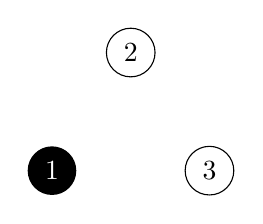
\begin{tikzpicture}
	\tikzset{every node/.style={circle, draw}}
\node[draw=none, fill=black, text=white] (n1) at (1,1) {$1$};
\node (n2) at (2,2.5) {$2$};
\node (n3) at (3,1) {$3$};

	\end{tikzpicture}
	\caption{$3K_1$ with Red move}
\end{figure}

Further, the edges of this graph represent the binary constraints enforced by
the game. Thus, the edges of the graph determine which sections of the graph to
update when a move is made i.e. when a unary constraint is enforced on a
vertex.

An edge, $(i, j)$ where $i, j \in \mathbf{V}$, may only exist in the graph if
exactly one of the following conditions hold: $i$ and $j$ are both labeled as
$\mathbf{A}$ or exactly one of $i$ and $j$ is labeled as $\mathbf{A}$.

\subsection{Making Moves}

A move is characterized by the following process:
\begin{enumerate}
	\item A player selects a vertex that is labeled by their color or
		$\mathbf{A}$.
	\item The vertex obtains the label $\mathbf{U}$.
	\item All neighboring vertices are recursively updated to maintain
	\emph{arc-consistency}.
\end{enumerate}

Arc-consistency\footnote{Although arc-consistency maintenance is usually an
expensive operation, $O(ed^3)$ through AC-3 \cite{0023820},
it can be shown that forward checking up to two vertices is sufficient due to
the nature of the binary constraints i.e.  $O(d^2)$.} is the state of the graph
in which $(\mathbf{X}, \mathbf{Y})\in\mathbf{E}$ is called consistent if
$x\in\mathbf{X}$ and $y\in\mathbf{Y}$ are consistent. The value,
$x\in\mathbf{X}$ is said to be consistent if and only if $x\in
dom(\mathbf{X})$.

\subsection{Terminal State Characterization}

\begin{defn}
	A game, $\mathbf{G}$, is in a terminal state, $\mathbf{G_t}$, if and only
	if there are no vertices with the label $\mathbf{A}$ and there are no
	binary edges.
\end{defn}

The terminal state has the property that a winner can be determined by the
currently labeled vertices and the current player's turn. It is important to
note that the set of gameover states is a subset of the set of terminal states.
Subsequently, we will end our analysis of a game at a terminal state because a
simple linear-time evaluation algorithm exists to evaluate the state.

The evaluation algorithm determines the \emph{game value}, $v$ of the state.
The game value represents the payoff for a specified player. Without loss of
generality, $v$ will represent the payoff of the Red player and $\overline{v}$,
the payoff for the Blue player, will simply be the negation of $v$ according the
rules of a zero-sum game.

The evaluation algorithm runs as follows:
\begin{enumerate}
	\item Initialize an accumulator to $0$.
	\item Add the number of $\mathbf{R}$-labeled vertices to the accumulator.
	\item Subtract the number of $\mathbf{B}$-labeled vertices from the accumulator.
	\item If the current game state is Blue's turn, add $\frac{1}{2}$ to the accumulator.
\end{enumerate}

According this evaluation algorithm, the following outcomes are possible
relative to $v$.
\begin{itemize}
	\item If $v > 0$, Red wins.
	\item If $v \leq 0$, Red loses.
	\item If $v = \frac{1}{2}$, Red wins by a single turn ahead.
\end{itemize}

Consider the following example in figure \ref{fig:3K_1-Terminal} where it is
the Red player's Turn. We begin with an accumulator $a = 0$. There is one
$\mathbf{R}$-labeled vertex, so we add one: $a = 1$. There is one
$\mathbf{B}$-labeled vertex, so we subtract one: $a = 0$.
\begin{figure}[h]
	\label{fig:3K_1-Terminal}
	\centering
	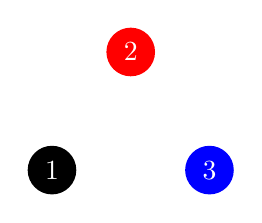
\begin{tikzpicture}
	\tikzset{every node/.style={circle, draw}}
\node[draw=none, fill=black, text=white] (n1) at (1,1) {$1$};
\node[draw=none, fill=red!, text=white] (n2) at (2,2.5) {$2$};
\node[draw=none, fill=blue!, text=white] (n3) at (3,1) {$3$};

	\end{tikzpicture}
	\caption{$3K_1$ Terminal State on Blue's Turn}
\end{figure}
The game is balanced, hence the next player to move will lose i.e. this is a
\ppos-position. Since it is the Blue player's turn, we add $\frac{1}{2}$.
Hence, $a = \frac{1}{2}$ and Red wins by a single turn ahead.

\section{Computability and Complexity Bounds Analysis}

Determining which player has a winning strategy is possible, though
intractable, since the game is progressively bounded i.e. a valid terminal
state will eventually be reached. Hence, the problem of determining which
player has a winning strategy is computable.

We can determine the upper-bound on the number of possible game states using a
constraint relaxation argument, because a game state can be completely
represented by a discrete planar graph with finite values. That is,
disregarding the conditions for which a vertex can obtain a label, a vertex has
one of four labels exclusively. Hence, a planar graph with $n$ vertices can
have at most $o(4^n)$ potential states which both valid states and invalid
states. 

\subsection{Unfairness}

We can determine the fairness of the game by showing that a winning strategy
exists for one of the players exclusively. For every game state, the game is
progressively-bounded and there are no ties. It follows that a winning strategy
exists for every game. Since a winning strategy exists for every game state,
the game is unfair.

Instead of solving for the winning player for arbitrary graphs, however, we
will solve for winning players of general graph families.

\section{General Graph Families}

For the following general families of graphs, we show empirical results which
suggest a generalized winning strategy for each family of graphs. The results
enables us to infer an optimal strategy for the winning player.

\begin{table}[ht!]
	\centering
	\begin{tabular}{| c | c | c | c |}
		\hline
		$k$ & $v$ of $\mathbf{K_{1,k}}$ & $v$ of $\mathbf{P_k}$ & $v$ of $\mathbf{C_k}$ \\\hline
		1	& 0.5	& 0.5	& 0.5	\\\hline
		2	& 1.5	& 1	 	& 1.5	\\\hline
		3	& 2.5	& 2	 	& 2.5	\\\hline
		4	& 3.5	& 1	 	& 0		\\\hline
		5	& 4.5	& 1	 	& 1		\\\hline
		6	& 5.5	& 0.5	& 0		\\\hline
		7	& 6.5	& 1.5	& 1		\\\hline
		8	& 7.5	& 1	 	& 0		\\\hline
		9	& 8.5	& 2	 	& 1		\\\hline
		10	& 9.5	& 1.5	& 0		\\\hline
		11	& 10.5	& 1.5	& 0.5	\\\hline
		12	& 11.5	& 1		& 0		\\\hline
	\end{tabular}
	\label{tab:emp}
	\caption{Empirical Game Values for Small Graphs}
\end{table}

We begin with the families of graphs for which a generalized winning strategy
is trivially known. When we outline a strategy, note that the Red player is the
first player without loss of generality.

	\subsection{Star Graphs}
	Star graphs of $k + 1$ vertices are denoted as $\mathbf{K_{1,k}}$.
	Trivially, selecting the center vertex is always the optimal strategy for
	the current player. Hence, all star graphs are \npos-positions.

	As an example of the trivial strategy, consider the claw graph:
	\begin{figure}[h]
		\centering
		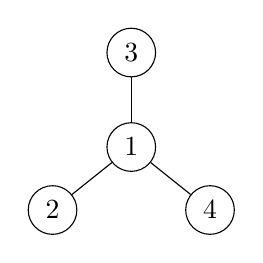
\begin{tikzpicture}[node distance=3cm]
		\tikzset{every node/.style={circle, draw}}
\node (n1) at (2,1.8) {$1$};
\node (n2) at (1,1) {$2$};
\node (n3) at (2,3) {$3$};
\node (n4) at (3,1) {$4$};

\foreach \from/\to in {n1/n2,n1/n3,n1/n4}
{
	\draw (\from) -- (\to);
}

		\end{tikzpicture}
		\caption{$\mathbf{Claw}$, N-Position}
	\end{figure}
	Selecting the center vertex will isolate the surrounding vertices and
	restrict their values from the opposing player's color.

	\eject
	\subsection{Path Graphs}
	Path graphs with $k$ vertices are denoted as $\mathbf{P_{k}}$. Path
	graphs contain $k - 1$ edges that create binary links between
	vertices similar to a linked list.
	
	Special points on the graph are defined as follows:
	\begin{defn}
		For all path graphs, $\mathbf{P_k}$ where $k \geq 3$, the leftmost vertex
		is said to be the head of the graph.
	\end{defn}
	\begin{defn}
		For all path graphs, $\mathbf{P_k}$ where $k \geq 3$, the rightmost vertex
		is said to be the tail of the graph.
	\end{defn}

	\begin{theorem}
		\label{thm:path}
		All path graphs, $\mathbf{P_k}$ with $k$ vertices are \npos-positions.
	\end{theorem}

	\begin{proof}
		To prove that theorem \ref{thm:path} holds, we must consider two cases:
		\begin{itemize}
			\item Every even-length path graph is an \npos-position.
			\item Every odd-length path graph is an \npos-position.
		\end{itemize}

		\begin{case}
		The optimal strategy for path graphs of even-length is as follows:
		\begin{enumerate}
			\item Red player selects the vertex neighboring the head or tail.
				Without loss of generality, we assume the head.
			\item The path graph disconnects into two subgraphs, $\mathbf{P_1},
				\mathbf{P_{k-2}}$.
			\item Blue player selects the vertex neighboring the leftmost
				$\mathbf{R}$-labeled vertex, $u$, on the larger subgraph such that the
				$u$ obtains label $\mathbf{U}$.
			\item Red player applies the same strategy as in step (3) such that
				the neither player will never have an game value advantage of
				greater than $\frac{1}{2}$. In the case of $\mathbf{P_4}$ with
				a $\mathbf{R}$-labeled head, the game value is $\frac{1}{2}$.
				In the case of $\mathbf{P_6}$ with a $\mathbf{R}$-labeled head,
				the game value is $-\frac{1}{2}$. All other even-length path
				graphs alternate this property.
			\item By the end of the game, regardless of which player has the advantage
				in the larger subgraph, the Red player already had a game value
				advantage of 1. Hence, the Red player always wins.
		\end{enumerate}
		\end{case}

		\begin{case}
		The optimal strategy for path graphs of odd-length is as follows:
		\begin{enumerate}
			\item Red player selects the center vertex.
			\item Blue player selects the vertex which shares a mutual neighbor
				from rightmost $\mathbf{B}$-labeled vertex or the head if no such
				vertex exists yet.
			\item Red player selects the vertex which shares a mutual neighbor
				from the leftmost $\mathbf{R}$-labeled vertex or the tail if no
				such vertex exists yet.
			\item Steps (2) and (3) repeat until the graph is completely
				disconnected in which case both players will have the same number
				of colored vertices; however, Blue had one turn ahead in selecting
				vertices on a symmetric game as seen in step (2).
			\item Hence, Blue will always lose i.e. Blue will be the next to move
				in the absolute gameover state.
		\end{enumerate}
		\end{case}

		Because the set of even-length path graphs union the set of odd-length
		path graphs encapsulates the entire set of path graphs, all path
		graphs, $\mathbf{P_k}$ where $k \geq 1$, are \npos-positions.
	\end{proof}

	Odd-length path graphs also yield the property that we call the
	\emph{odd-rule}.
	\begin{defn}
		For all path graphs, $\mathbf{P_k}$ where $k$ is odd, the odd-rule
		states that $\mathbf{P_k}$ will end on the opposing player's turn such
		that the current player will move afterwards if the game state were to
		continue.
	\end{defn}

	\begin{remark}
		Assuming that the leftmost vertex is blue and the rightmost vertex is
		red without loss of generality, the odd-rule holds.
	\end{remark}

	\subsection{Cycle Graphs}
	A cycle graph, $\mathbf{C_k}$, has $k$ vertices with edges $(i, i+1
	\pmod{k})$ for $i\in[0,k]$. For cycle graphs with $k>3$, the winning
	player alternates.
	\begin{theorem}
	For a cycle graph, $\mathbf{C_k}$ where $k>3$, if $k$ is even, $\mathbf{C_k}$ is a \ppos-position.
	\end{theorem}

	Beware that $\mathbf{C_4}$ is a special case that decomposes into
	$\mathbf{K_3}$ for Blue player. As an illustration of the strategy, see figure
	\ref{fig:c4}. Red player selects any vertex without loss of generality.
	\begin{figure}[h]
		\label{fig:c4}
		\centering
		\begin{tikzpicture}[node distance=3cm]
		\input{cycle-4-graph}
		\end{tikzpicture}
		\caption{$\mathbf{C_4}$, P-Position}
	\end{figure}
	Blue player has only one option: choose the vertex across from it. Once the
	vertex has been selected, all of Red player's options become void. Hence,
	Blue player always wins.

	The strategy for all even-sized cycle graphs where $k \geq 6$ decomposes a
	cycle-graph into two equal-length path-graphs,
	$2\mathbf{P_{\frac{k-2}{2}}}$. The strategy is as follows.
	\begin{enumerate}
		\item Red player selects a vertex without loss of generality.
		\item Blue player selects the vertex directly across from it.
		\item Two path graphs of same size are generated.
		\item Since it is Red player's turn, we have shown that the first to move
			in the path graph always wins.  Hence, Red player wins the first
			path graph.
		\item Since Red player wins the first path graph, it follows that Blue player
			begins the second path graph. Hence, Blue player wins the second path
			graph.
		\item By symmetry, any game value, $v$, obtained by the Red player on
			the first graph is obtained by the Blue player as $\overline{v}$.
			Consequently, the total game value is $v + \overline{v} = 0$.
			Consequently, the Blue player wins.
	\end{enumerate}
	Note that after step (1), the odd-rule applies which simplifies the proof;
	however, the roles of the Red and Blue player are reversed and thus, the
	Red player will always lose.

	\begin{theorem}
	For a cycle graph, $\mathbf{C_k}$ where $k>3$, if $k$ is odd,
	$\mathbf{C_k}$ is an \npos-position.
	\end{theorem}

	\begin{figure}[h]
		\label{fig:c5}
		\centering
		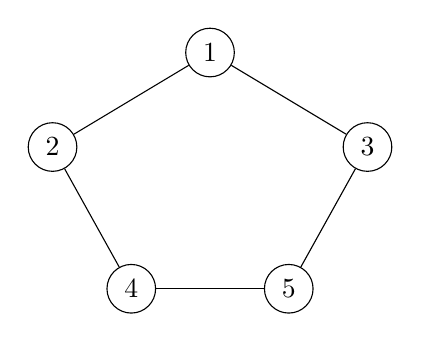
\begin{tikzpicture}[node distance=1cm]
		\tikzset{every node/.style={circle, draw}}
\node (n1) at (3,3) {$1$};
\node (n2) at (1,1.8) {$2$};
\node (n3) at (5,1.8) {$3$};
\node (n4) at (2,0) {$4$};
\node (n5) at (4,0) {$5$};

\foreach \from/\to in {n1/n2,n1/n3,n2/n4,n3/n5,n4/n5}
{
	\draw (\from) -- (\to);
}

		\end{tikzpicture}
		\caption{$\mathbf{C_5}$, N-Position}
	\end{figure}
	The idea behind the strategy is that any vertex selected reduces the game
	to an even-sized path graph, $\mathbf{P_{k-1}}$ with a head and tail of the
	same label as the current player. On the following move, the path graph is
	broken into two smaller graphs which are even and odd in length. The odd
	graph has a special property which enforces a turn advantage.
	\begin{figure}[h]
		\label{fig:P4-Head-Tail}
		\centering
		\begin{tikzpicture}[node distance=1cm]
		\input{P_4-Head-Tail}
		\end{tikzpicture}
		\caption{$\mathbf{P_4}$ with Red Head and Tail, P-Position}
	\end{figure}
	The strategy is as follows:
	\begin{enumerate}
		\item Red player selects a vertex without loss of generality.
		\item The graph unfolds into a path graph with $k-1$ vertices,
			$\mathbf{P_{k-1}}$ i.e. even-sized (see figure \ref{fig:P4-Head-Tail}).
		\item Blue player selects one of two center vertices in the path graph
			without loss of generality.
		\item The graph unfolds into a two path graphs of size $\lceil\frac{k -
			2}{2}\rceil$ and $\lfloor\frac{k - 2}{2}\rfloor$ each with a game
			value of zero. The two path graphs have the property that one is odd-length and the
			other is even-length. By the odd-rule, the Red player can choose
			the odd-length such that it is the Red player's turn to start the
			even-length game. Further, because all even-length graphs are
			\npos-positions, the Red player wins the even-length game. Because
			all subgames have been solved, the Red player wins.
	\end{enumerate}

\section{Game Variation by Players}

It is due to the number of players that the complexity of the game grows
exponentially. Recall that that number of labels is also the number of subsets
of all possible values that can be obtained by a vertex. We begin by noting
that there the $\mathbf{A}$ and $\mathbf{U}$ labels are always required.
However, for $n$ players, there are $n + 2$ possible values. Hence, the size of
the state space becomes $o((n+2)^{|V|})$ where $|V|$ is the number of vertices
of a specified map.

Trivially, the star graph family will always be an \npos-position regardless of
the number of players.

\section{Conclusion}

We have shown that for non-cycle, graphs, the game of Snort is almost always
biased towards the first player. On our simulation, we randomly-generated
graphs through an Erd\H{o}s-R\'{e}nyi algorithm of vertex range $(5, 13)$ and
edge probability of $0.2$. Through $100$ games using a minimax solver, it was
seen that almost all games had winning strategies by the first player. Due to
the immense state space size, graphs larger than $13$ often took longer than 30
minutes to solve.  Subsequently, a practical heuristic, if state-space search
is intractable, is to select vertices of high-degree. 

We have also shown a proof of the tractability of cycle graphs shows that
proofs of tractability can be created for composite graphs i.e.  graphs
composed of several, simpler graphs. Hence, there are several open questions
available regarding the tractability of other special cases of composite graphs
using simple graph reductions.

\bibliographystyle{plain}
\bibliography{science,dblp}

\end{document}
